\chapter{Approach}\label{chap:approach}
In order to investigate the use of explicit semantic representations for the task of local citation recommendation we first need to decide which kinds of semantic constructs we want to model. As a starting point for this we looked into the field of citation context analysis~\cite{HERNANDEZ-ALVAREZ2016}. A common task in this area is the classification of citation contexts by their polarity (positive/neutral/negative) and function (often based on the four dimensions identified by Moravcsik et al.~\cite{Moravcsik1975}, conceptual/operational, evolutionary/juxtapositional, organic/perfunctory, conformative/negational). Such approaches are primarily concerned with the \emph{intent} of the author rather than the \emph{content} of what is being cited. We can therefore not expect to derive types of semantic constructs directly from citation functions. Starting from an established typology of citation functions will, however, ensure that we consider a wide range of different citations rather than cherry picking those that fit our preconceptions.

\begin{table}[]
\centering
    \caption{Semantic constructs in citation contexts from a range of citation functions used in the field of citation context analysis.}
    \label{tab:citfunctions}
\begin{center}
    \begin{tabular}{m{2.7cm}lm{8.5cm}}
    \toprule
    Function & Construct & Examples (semantic construct \emph{highlighted})\\
    \midrule
    Attribution & claim & ``Berners-Lee et al.~\cite{Berners-Lee2001} argue that \emph{structured collections of information and sets of inference rules are prerequesites for the semantic web to function}.'' \\\noalign{\smallskip}
    \  & NE & ``A variation of this task is `\emph{context-based co-citation recommendation}'~\cite{Kobayashi2018}.'' \\\noalign{\smallskip}
    \  & - & ``In \cite{Duma2014} Duma et al. test the effectiveness of using a variety of document internal and external text inputs to a TF-IDF model.'' \\\noalign{\medskip}
    Exemplification & NE & ``We looked into approaches to \emph{local citation recommendation} such as~\cite{He2010,Huang2014,Huang2015,Duma2014,Duma2016,Ebesu2017,Kobayashi2018,Jeong2019} for our investigation.'' \\\noalign{\medskip}
    Further reference & - & ``See \cite{Niklaus2018} for a comprehensive overview.'' \\\noalign{\medskip}
    Statement of use & NE & ``We use \emph{CiteSeerX}~\cite{Caragea2014} for our evaluation.'' \\\noalign{\medskip}
    Application & NE & ``Using this mechanism we perform `\emph{context-based co-citation recommendation}'~\cite{Kobayashi2018}.'' \\\noalign{\medskip}
    Evaluation & - & ``The use of DBLP in \cite{Faerber2018} restricts their data set to the field of computer science.'' \\\noalign{\medskip}
    Establishing links between sources& claim & ``A common motivation brought forward for research on citation recommendation is that \emph{finding proper citations is a time consuming task} \cite{He2010,He2011,Ebesu2017,Kobayashi2018}.'' \\\noalign{\smallskip}
    \  & - & ``Lamers et al.~\cite{Lamers2018} base their definition on the author's name whereas Thompson~\cite{Thompson2001} focusses on the grammatical role of the citation marker.'' \\\noalign{\medskip}
    Comparison of own work with sources& claim & ``Like \cite{Faerber2018} we find that, albeit written in a structured language, \emph{parsing \LaTeX{} sources is a non trivial task}.'' \\
    \bottomrule
    \end{tabular}
\end{center}
\end{table}

Table~\ref{tab:citfunctions} lists categories of citation functions along with the kinds of semantic constructs that can be found in such citation contexts. The list of citation functions is taken from \cite{Petric2007} (and therein built upon \cite{Thompson2001}). This study was selected because it gives an overview of previous attempts to classify citations, presents their new typology with extensive explanation as well as example contexts, and does not mix polarity into its function categories. Examining contexts from each of the eight functions we identify two types of semantic constructs: named entities (NE) and claims (or statements). The rationale behind these two is as follows. Named entities can identify reference publications for a certain data set/tool/concept (see \emph{Attribution}, \emph{Statement of use} and \emph{Application} in Table~\ref{tab:citfunctions}) as well as a method/field of study common to a selection of publications (see \emph{Exemplification} in Table~\ref{tab:citfunctions}). Claims can identify publications that can be cited to back or support the very claim contained in a citation context. Note that the example contexts listed to have no construct (``-'' in the \emph{Construct} column) may contain named entities and claims as well (e.g. ``DBLP'' or ``Lamers et al. base their definition of the author's name''), but these are (in the case of NEs) not representative of the cited work or (in the case of claims) just statements \emph{about} a publication rather than statements being backed by the cited work.
A third semantic construct that can be considered, but would require considering a larger citation context, is argumentative structures. To keep the scope of this thesis at a reasonable level we will, however, limit our investigation to named entities and claims.

The following sections will describe our investigation of entity based and claim based models for local citation recommendation.

\section{Entity based recommendation}
The intuition behind an entity based approach is, that there exists a reference publication for a named entity. Examples would be a data set (``CiteSeerX~\cite{Caragea2014}''), a tool (``Neural ParsCit~\cite{Animesh2018}'') or a concept (``Semantic Web~\cite{Berners-Lee2001}''). In a more loose sense this can also include publications being referred to as examples (``approaches to local citation recommendation~\cite{He2010,Huang2014,Huang2015,Duma2014,Duma2016,Ebesu2017,Kobayashi2018,Jeong2019}'').
% mention DBpedia Spotlight tests? (sufficient data available?)
For the identification of such named entities we take two approaches. A more strict one based on the fields of study given in the MAG, and a more loose one based on noun phrases.

\subsection{Fields of study in the MAG}\label{sec:approachfos}
Along with papers, authors, venues etc. the MAG data schema also includes fields of study (FoS) that are associated with papers and interlinked in a child-parent manner. At the time of writing there are 229,716 FoS at 6 levels of granularity. They range from the most coarse level 0 (example entries being \emph{mathematics}, \emph{sociology},  \emph{computer science}) to more and more fine grained entities (\emph{information retrieval}$_{(1)}$→\emph{search engine}$_{(2)}$→\emph{web search query}$_{(3)}$→\emph{ranking (information retrieval)}$_{(4)}$→\emph{Okapi BM25}$_{(5)}$). The levels of granularity don't seem to follow a globally consistent pattern though. \emph{WordNet}, for example, being a particular piece of data in the same way \emph{Okapi BM25} is a particular function, is not at level 5 but level 2 (\emph{computer science}$_{(0)}$→\emph{artificial intelligence}$_{(1)}$→\emph{WordNet}$_{(2)}$). Another noteworthy aspect is that a FoS can have multiple parents (\emph{search engine} for example has a second parent in \emph{World Wide Web}).

\paragraph{Model} The entity based representation of a citation context is the set of FoS that appear within the context. Formally, let $\mathcal{F}$ denote the set of FoS; then the entity based representation of a citation context $c$ is the set of terms $t$ defined as ${R_{\text{FoS}}(c) = \{t|t\text{ appears in }c \land t\in \mathcal{F}\}}$. Because of the hierarchical structure of FoS we experiment with augmenting the set by including the set members' parents into the representation. We find that his leads to worse results, presumably because a context's description becomes more vague which is detrimental to identifying reference publications or exemplifications. We furthermore look into only using a FoS when it directly precedes the citation marker---as it might be more relevant to the citation then---, but notice that such cases are too rare. In a preliminary test with 900k citation contexts, only 0.14\% of our 180k test set items have a FoS in the required position matching any of the representations learned from the training set.

\paragraph{Recommendation} For recommending documents based on $R_{\text{FoS}}$ we use the Jaccard similarity between the input citation context and the aggregrated citation contexts describing each candidate document. Formally, let $c_i$ denote the input citation context and $\mathcal{D}$ be a set of documents with members $d\in \mathcal{D}$. Furthermore let $\varrho(d)$ be the set of citation contexts referencing $d$; ${\varrho(d)=\{c|c\text{ references } d\}}$. The Jaccard similarity then is defined as ${J(A,B)=\frac{|A\cap B|}{|A\cup B|}}$, where $A = R_{\text{FoS}}(c_i)$ and $B=\bigcup\limits_{c \in \varrho(d)} R_{\text{FoS}}(c)$.

\subsection{Noun phrases}\label{sec:npmodel}
For our second entity based model we take a more loose approach and treat noun phrases extracted from the arXiv data set as named entities. By filtering out items that appear only once we end up with 2,835,929 noun phrases (NPs).

\paragraph{Model} Similar to the FoS representation, we look at the NPs appearing within a citation context. To ensure a high descriptiveness, we only take into account maximally long matches. A context \emph{``This has been done for language model training [27]''}, for example, would have ``language model training'' in its representation, but not ``language model''. Formally we can define ${R_{\text{NP}}(c) = \{t|t\text{ appears in }c \land t\in \mathcal{P} \land t^{+pre} \notin \mathcal{P}\land t^{+suc} \notin \mathcal{P}\}}$ where $\mathcal{P}$ is our set of NPs while $t^{+pre}$ and $t^{+suc}$ denote an extension of $t$ using its preceding or succeeding word respectively. As an alternative representation we furthermore define ${R_{\text{NPmrk}}^{2+}(c)}$ as a subset of ${R_{\text{NP}}(c)}$ containing, if present, the NP of minimum word length 2 directly preceding the citation marker in $c$ that a prediction is to be made for. Formally, ${R_{\text{NPmrk}}^{2+}(c) = \{t|t\in R_{\text{NP}}(c)\land len(t)\geq 2 \land t\text{ directly precedes } m\}}$ where $m$ is the citation marker in $c$ that a prediction is to be made for.

\paragraph{Recommendation} Recommending documents based on ${R_{\text{NP}}}$ and ${R_{\text{NPmrk}}^{2+}}$ is done using a vector space model (VSM) in which NP representations, treated as a bag of word (BoW), are compared by their cosine similarities. Representations of candidate documents are, likewise to the FoS based model, aggregrates over all contexts referencing the document. Formally, the vector representation of a context is given by $V(R(c)) = (t_{1,j}, t_{2,j}, ..., t_{|\mathcal{P}|,j})$ where $\mathcal{P}$ is the set of all NPs % technically wrong b/c sets are not ordered
and $t_{i,j}$ is a non-negative integer representing a quantity with regards to the $i$th term in $\mathcal{P}$. Aggregated context representations for candidate documents are caluclated by adding up all vector representations of the contexts referring to a document. I.e., let $\varrho(d)$ be the set of citation contexts referencing $d$, then $d$'s vector representation is $\sum\limits_{c \in \varrho(d)} V(R(c))$. The similarity between an input context $c_i$ and a candidate document $d\in \mathcal{D}$ can then be calculated as the cosine $\theta$ between the two vector representations ${\mathrm{cos}(\theta)=\frac{A\cdot B}{\|A\| \|B\|}}$ where  $A=V(R(c_i))$ and $B=\sum\limits_{c \in \varrho(d)} V(R(c))$.

\section{Claim based recommendation}
%For the introduction of a claim based model we first need to make a few observations on how citations interact with the text they're placed in. By convention, citations are constructed by placing a type of marker, which identifies an entry in the document's reference section, in the text. These markers can, depending on discipline, journal, etc. take different forms. Some examples are numbers in square brackets (``In [27] ...''), alphanumeric identifiers in square brackets (``In [Bol98] ...''), a year in parentheses succeeding an author's name (``Swales (1990) has argued ...'') and an author's name with a year in parentheses (``It has been argued (Swales, 1990) ...''). Named entities can stand in a grammatical relation to such a marker. In ``By using CiteSeer, [Bol98], we ...'', for example, the named entitiy \emph{CiteSeer} and the citation marker \emph{[Bol98]} are in a grammatical relation called \emph{apposition}. A citation marker can, however, reasonably assumend to never be \emph{part of} the named entity. This is different in the case of the statements within a citaiton context. Looking at the sentence ``In \cite{Bollacker1998} Bollacker et al. introduce Citeseer.'' we can see that the marker itself is part of what is being said, while this is not the case in, for example, ``Bollacker et al. introduced Citeseer in 1998~\cite{Bollacker1998}.''. Citations w
For the introduction of a claim based model we first need to make a few observations on how citations interact with the text they're placed in. Citing is done by placing a citaiton marker (that has a corresponding entry in the reference section) in the text. Such a marker is sometimes put into a sentence such that it functions as a word (e.g. ``In \cite{Bollacker1998} Bollacker et al. introduce Citeseer.'' or ``For further details see \cite{Bollacker1998}.'') and sometimes detached from the sentence's grammatical structure (e.g. ``Bollacker et al. introduced Citeseer in 1998~\cite{Bollacker1998}.'' or ``CiteSeer~\cite{Bollacker1998} was introduced in 1998.''). Put differently, in the latter two examples the sentences work just fine without the citation markers (``Bollacker et al. introduced Citeseer in 1998.'', ``CiteSeer was introduced in 1998.'') while the former two become ungrammatical or change in meaning (``In Bollacker et al. introduce Citeseer.'', ``For further details see.''). As suggested in \cite{Whidby2011} and \cite{Abujbara2012}, we will refer to citations where the citation marker has a grammatical function as ``syntactical'', and to ones where the citation marker is not part of the actual setence as ``non-syntactical''  (a more detailed discussion of this and related terminology can befound in Appendix~\ref{chap:integralsyntactic}). This distiction will be relevant because claims within a citation context can, in the case of syntactical citations, be in a grammatical relation to or even contain citation markers.

The following sections will describe our evaluation of tools for extracting claims from citation contexts and the model we developed for recommendation.

\subsection{Tools for extracting claims}
For the extraction of claims we consider a total of four state of the art \cite{Zhang2017} information extraction tools: PredPatt~\cite{White2016}, Open IE 5.0~\cite{Mausam2016}, ClausIE~\cite{DelCorro2013} and Ollie~\cite{Mausam2012}. All of these can identify information in unformatted text, which they output in some form of predicate-argument tuples. Listing~\ref{lst:ietools} shows the output of all four tools for the simple sentence \emph{``The paper shows that context-based methods can outperform global approaches.''}.

\begin{lstlisting}[caption={Information extraction tool output examples.},label={lst:ietools}]
# PredPatt
?a shows ?b
    ?a: The paper
    ?b: SOMETHING := context-based methods can outperform global approaches
?a can outperform ?b
    ?a: context-based methods
    ?b: global approaches

# Open IE 5.0
0.90 Context(The paper shows,List([0, 15))):(context-based methods; can outperform; global approaches)
0.78 (The paper; shows; that context-based methods can outperform global approaches)

# ClausIE
"The paper" "shows" "that context-based methods can outperform global approaches"
"context-based methods" "can outperform" "global approaches"

# OLLIE
0.659: (context-based methods; can outperform; global approaches)[attrib=The paper shows]
\end{lstlisting}

Because the output for simple sentences is comarable for all of the tools, we tested them on 5 non trivial citation contexts, each consisting of 3 sentences. Based on this evaluation---the details of which are given in Appendix~\ref{chap:claimextooleval}---we deem PredPatt to perform the best, which is consistent with the observations in \cite{Zhang2017}.

% also: Survey on open information extraction\cite{Niklaus2018}

% context specific claim detection\cite{Levy2014}

% if only papers where semantically annotated as proposed in \cite{BuckinghamShum2000}
\subsection{A predicate-argument model}
Starting out with the predicate-argument tuples as PredPatt outputs them, we tested if there was enough of an overlap betweeen the components among citation contexts to facilitate recommendation. Taking the example from Listing~\ref{lst:ietools}, we would note the predicates \emph{``show''} and \emph{``can outperform''} as well as the arguments \emph{``The paper''}, \emph{``context-based methods can outperform global approaches''}, \emph{``context-based methods''} and \emph{``global approaches''}. Even when not preserving the associations between predicates and their arguments---e.g. looking for other contexts where \emph{``global approaches''} was identified without requiring it to be in conjunction with \emph{``can outperform''}---, we note very little overlap between citation contexts. We believe this to be the case because the predicates and especially arguments that PredPatt identifies can get very long, like \emph{``can outperform''} (including the auxilliary verb \emph{``can''}) and \emph{``context-based methods can outperform global approaches''} (unlikely to appear in another citation context with the exact same wording).

\begin{figure}
  \centering
    \subfloat[Main clause.]{{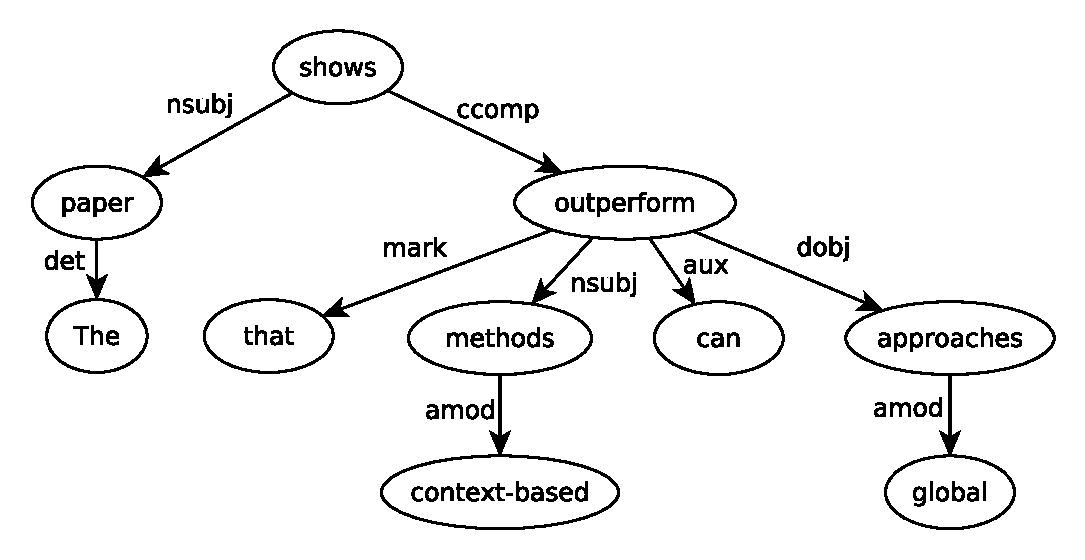
\includegraphics[width=.55\textwidth]{figures/approach/pp_tree0.pdf}}\label{fig:pptrees0}}
    \subfloat[Sub clause.]{{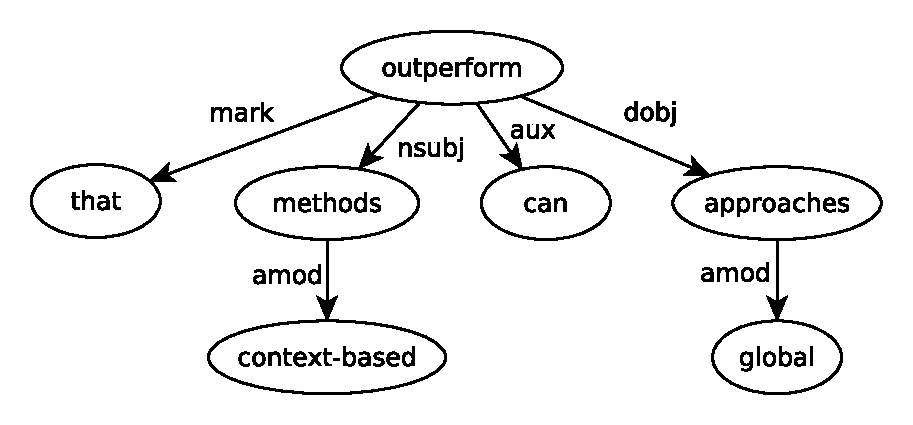
\includegraphics[width=.45\textwidth]{figures/approach/pp_tree1.pdf}}\label{fig:pptrees1}}
  \caption{UD trees as generated by PredPatt.}
  \label{fig:pptrees}
\end{figure}

To overcome this problem we develop a derivate model based on PredPatt's internal representation of sentences. Internally, PredPatt represents sentences in a tree structure based on Universal Dependencies (UD)~\cite{Nivre2016} (i.e. a dependency grammar as opposed to a constituency grammar). This means words are connected by directed edges where the source is referred to as \emph{governor}, the target is referred to as \emph{dependant} and the edge itself is associated with a type of \emph{relation}. Looking at Figure~\ref{fig:pptrees}, depicting PredPatt's internal view on the example sentence given in Listing~\ref{lst:ietools}, we can, for example, see that the \emph{``can''} is a dependant to and governed by \emph{``outperform''} in an auxilliary relation. How our (predicate-argument based) claim model is constructed from this tree structure and used for recommendation will be discussed in the following sections.

\begin{algorithm}
\caption{Construction of $R_{\text{claim}}(c)$}
\label{alg:pprep}
\begin{algorithmic}
    \State $c \gets \mathit{strip\_quotation\_marks}(c)$     \alignedComment{remove quotation marks}
    \State $c \gets \mathit{merge\_citation\_markers}(c)$     \alignedComment{e.g. ``CIT , CIT''→``CIT''}
    \State $\mathit{pp\_trees}_c \gets \mathit{predpatt}(c)$     \alignedComment{get PredPatt output}
    \State $\mathit{output} \gets []$     %\alignedComment{empty array}
    \State $\mathit{resolve\_rels} \gets [\text{'name'},\text{'goeswith'},\text{'mwe'},$     \alignedComment{\textbf{(b$_\mathbf{1}$)} UD relations}
    \State $\hphantom{\mathit{resolve\_rels} \gets [}\text{'compound'},\text{'conj'},\text{'amod'},$
    \State $\hphantom{\mathit{resolve\_rels} \gets [}\text{'advmod'}]$
    \ForEach{$t\in\mathit{pp\_trees}_c$}   \alignedComment{for all claims identified}
        \State $\mathit{root} \gets \mathit{get\_root}(t)$   %\alignedComment{get predicate}
        \State $\mathit{pred} \gets \mathit{identify\_predicate}(t)$   \alignedComment{\textbf{(a)} resolve copula if present}
        \State $\mathit{pred} \gets \mathit{lemmatize}(\mathit{pred})$   %\alignedComment{lemmatize}
        \ForEach{$n\in\mathit{traverse}(t)$}    %\alignedComment{traverse all nodes}
            \If{$\mathit{pos\_tag}(n) == \text{'NOUN'}$}   %\alignedComment{if it's a noun}
                \State $\mathit{arg} \gets \mathit{resolve\_all}(n, \mathit{resolve\_rels})$   \alignedComment{\textbf{(b$_\mathbf{2}$)} resolve compounds etc.}
                \State $\mathit{output.append}(\mathit{pred}+\text{':'}+\mathit{arg})$   \alignedComment{build pred:arg tuple}
            \EndIf
        \EndFor
    \EndFor\\
    \Return{$\mathit{output}$}
\end{algorithmic}
\end{algorithm}

\paragraph{Model} The construction of our claim representation $R_{\text{claim}}(c)$ for a citation context $c$ is shown in Algorithm~\ref{alg:pprep}. There are two preprocessing steps prior to applying PredPatt. Quotation marks matching the regular expression \texttt{[“”„"«»‹›$\mathtt{\langle\hspace{-1mm}\langle\rangle\hspace{-1mm}\rangle\langle\rangle}$]} are removed to avoid parsing errors, and groups of citation marker replacement tokens (e.g. \emph{``CIT , CIT , CIT''} originating from e.g. \emph{``[3,27,42]''}) are merged into one (i.e. \emph{``CIT''}) to get a cleaner and easier to parse sentence structure. After applying PredPatt, the UD tree of each of the identified claims is traversed and predicate-argument tuples are generated. A claim is always centered around a predicate, which is the root of the corresponding UD tree unless a compula (\emph{be}, \emph{am}, \emph{is}, \emph{are}, \emph{was}) is used, in which case the predicate is a dependant of the root node with the relation type \emph{``cop''} (this is handled at marker \textbf{(a)} in Algorithm~\ref{alg:pprep}). Once identified, predicates are lemmatized using NLTKs WordNetLemmatizer. For the identification of useful arguments (markers \textbf{(b$_\mathbf{1}$)} and \textbf{(b$_\mathbf{2}$)} in Algorithm~\ref{alg:pprep}), we look at all nouns within the UD tree and resolve compounds (\emph{``compound''}, \emph{``mwe''}, \emph{``name''} relations), phrases split by formatting (\emph{``goeswith''}), conjunctions (\emph{``conj''}) as well as adjectival and adverbial motifiers (\emph{``amod''}, \emph{``advmod''}). To give an example, the noun \emph{``methods''} in both trees in Figure~\ref{fig:pptrees} has the adjectival modifier \emph{``context-based''}. In such a case our model would not choose \emph{``methods''} as an argument to \emph{``outperform''} but \emph{``context-based methods''}. Listing~\ref{lst:ppmodel} shows the complete representation generated for the example sentence.

\begin{lstlisting}[caption={An example of $R_{\text{claim}}(c)$.},label={lst:ppmodel}]
[
 'show:paper',
 'show:context based methods',
 'show:global approaches',
 'outperform:context based methods'
 'outperform:global approaches',
]
\end{lstlisting}

As becomes apparent when looking at Listing~\ref{lst:ppmodel}, we do not preserve the order of arguments. I.e., instead of constructing a triple (e.g. \texttt{context based methods:outperform:global approaches}) we build two tuples (\texttt{outperform:context based methods} and \texttt{outper\-form:global approaches}). This sequential invariance means a certain loss in precision, but also allows us to capture the similarity between active voice and passive voice sentences without the need to ensure reliabe parsing of such grammatical constructs. The input \emph{``The paper shows that global approaches can be outperformed by context-based methods.''}, for example, also has the claim representation shown in Listing~\ref{lst:ppmodel}.

\paragraph{Recommendation} To make use of $R_{\text{claim}}$ for recommendation we use a VSM where each dimension is a predicate-argument tuple. Similarities within this VSM are calculated as cosines between TFIDF-weighted vectors. Formally, the vector representation of a context is given by $V(R(c)) = (t_{1,j}, t_{2,j}, ..., t_{|\mathcal{T}|,j})$ where $\mathcal{T}$ is the set of all predicate-argument tuples % technically wrong b/c sets are not ordered
and $t_{i,j}$ is a non-negative integer representing a quantity with regards to the $i$th tuple in $\mathcal{P}$. TFIDF values for each $t_{i,j}$ in $V(R(c))$ with respect to a collection of contexts $\mathcal{C}$ are calculated as $\mathit{TFIDF}(t, c, \mathcal{C}) = \mathit{tf}_{t,c} \times \mathit{idf}_{t,\mathcal{C}}$, where $\mathit{tf}_{t,c}$ denotes the number of occurences of $t$ in $c$, and $\mathit{idf}_{t,\mathcal{C}} = \mathit{log}\frac{|\mathcal{C}|}{|\{c\in\mathcal{C}|t\text{ appears in }c\}|}$ is the log of the number of contexts over the number of contexts containing $t$.

Likewise to ${R_{\text{NP}}}$, aggregated context representations for candidate documents are caluclated by adding up all vector representations of the contexts referring to a document. Again, let $\varrho(d)$ be the set of citation contexts referencing $d$, then $d$'s vector representation is $\sum\limits_{c \in \varrho(d)} V(R(c))$. The similarity between an input context $c_i$ and a candidate document $d\in \mathcal{D}$ can then be calculated as the cosine $\theta$ between the two vector representations ${\mathrm{cos}(\theta)=\frac{A\cdot B}{\|A\| \|B\|}}$ where  $A=\mathit{TFIDF}(V(R(c_i)))$ and $B=\mathit{TFIDF}\Big(\sum\limits_{c \in \varrho(d)} V(R(c))\Big)$.

% As a variation, we also define a model that combines $R_{\text{claim}}$ similarities with BoW similarities.

% predicates could be grouped/clustered to represent functions as in \cite{Gabor2018}

% alternative view: model gives a selective citation context derived from claim structure (cf. concept of reference scope as sub part of citation context sentence\cite{Abujbara2012,RAHUL2017}
